\chapter{Javadoc}
\renewcommand{\chaptertitle}{Javadoc}

\lehead[]{\sf\hspace*{-2.00cm}\textcolor{white}{\colorbox{lightblue}{\makebox[1.60cm][r]{\thechapter}}}\hspace{0.17cm}\textcolor{lightblue}{\chaptertitle}}
\rohead[]{\textcolor{lightblue}{\chaptertitle}\sf\hspace*{0.17cm}\textcolor{white}{\colorbox{lightblue}{\makebox[1.60cm][l]{\thechapter}}}\hspace{-2.00cm}}
%\chead[]{}
\rehead[]{\textcolor{lightblue}{AvHG, Inf, My}}
\lohead[]{\textcolor{lightblue}{AvHG, Inf, My}}

\lstset{style=myJava}

Um in größeren Programmen nicht den Überblick zu verlieren, und um fremde
Klassen effizient nutzen zu können, ist es unerlässlich die Klassen, ihre
Attribute und Methoden zu dokumentieren.

Dies könnte klassisch in einem separaten Dokument getan werden. Java bietet für
diesen Zweck jedoch mit {\em Javadoc} eine Möglichkeit, die Kommentare direkt im
Quelltext unter zu bringen.

Aus diesen Javadoc-Kommentaren lässt sich anschließend Dokumentation in
verschiedenen Formaten (unter anderem HTML, RTF und PDF) automatisiert
erstellen.

Für den Programmierer besonders nützlich ist jedoch, dass diese Kommentare in
Eclipse (und anderen Entwicklungsumgebungen) dazu genutzt werden, um schon beim
Arbeiten mit Java-Quelltexten die entsprechenden Hinweise geben zu können --
etwa wenn man mit der Maus über einer entsprechenden Methode schwebt.


\section{Javadoc als Sonderfall von Kommentaren}

Technisch gesehen sind Javadoc-Kommentare ein Sonderfall von Kommentaren in
Java-Quelltexten. Zur Erinnerung:

\begin{lstlisting}
// Mit dem doppelten Forward-Slash wird der Rest der Zeile zum Kommentar.

/* 
 * Mehrzeilige Kommentare:
 *
 * Entscheidend sind nur die Markierungen der ersten und der letzten Zeile des
 * Kommentars. Die dazwischen liegenden Zeilen müssen nicht mit einem Asterisk
 * (Sternchen) markiert werden.
 */
\end{lstlisting}

Ein Javadoc-Kommentar ist ein Sonderfall des mehrzeiligen Kommentars: Zur
Unterscheidung wird der Javadoc-Kommentar mit \lstinline|/**| statt mit
\lstinline|/*| eingeleitet:

\begin{lstlisting}
/**
 * Dieser Kommentar wird als Javadoc-Kommentar interpretiert.
 */
\end{lstlisting}


\section{Javadoc zum Dokumentieren von Klassen, globalen Variablen und Methoden}

Mit Javadoc können nicht beliebige Programmelemente kommentiert werden. So ist
es beispielsweise nicht möglich, eine \lstinline|for|-Schleife mit Javadoc zu
kommentieren.

Der Sinn von Javadoc ist die Dokumentation von Schnittstellen einer Klasse.
Interna der Programmierung hingegen sind nicht das Ziel von Javadoc.

Konkret lassen sich folgende Elemente eines Java-Programms mit
Javadoc-Kommentaren versehen:

\begin{compactitem}
\item Die Klasse selbst
\item globale Variablen der Klasse (Klassen- und Objektvariablen)
\item Methoden
\end{compactitem}

Aus dem oben genannten Grund sind lokale Variablen nicht mit Javadoc zu
dokumentieren.


\section{Javadoc-Tags}

Je nach Kontext (Klasse, Methode oder Variable) stehen einem verschiedene Tags
zur Verfügung, etwa um die Bedeutung von Parametern zu beschreiben.

Die für uns wichtigsten Tags sind:

\bgroup
\def\arraystretch{1.2}
\begin{tabularx}{\textwidth}{|X|p{60mm}|p{25mm}|}\hline
%\begin{tabular}{|l|l|l|}\hline
\textbf{Tag \& Parameter} & \textbf{Bedeutung} & \textbf{Kontext} \\ \hline
\lstinline|@author name| & Name des Autors & Klasse, Interface \\ \hline
\lstinline|@param name description| & Parameterbeschreibung einer Methode
& Methode \\ \hline 
\lstinline|@return description| & Beschreibung des Rückgabewertes einer Methode
& Methode \\ \hline
\lstinline|@throws classname description| & Beschreibung einer Exception, die
von einer Methode erzeugt werden kann & Methode \\ \hline
\end{tabularx}
\egroup

Siehe

\url{http://de.wikipedia.org/wiki/Javadoc}


\section{HTML-Formatierungen}

Die Javadoc Kommentare werden als HTML interpretiert und angezeigt. Das bedeutet
auch, dass man HTML-Tags zur Formatierung benutzen kann.

So können beispielsweise Absätze mit \lstinline|<p>| und \lstinline|</p>|
eingefasst werden.

Klassen-, Methoden- und Variablen-Namen (und auch sonstiger Java-Quelltext) kann
mit \lstinline|<code>| und \lstinline|</code>| eingefasst werden.

Grundsätzlich können alle HTML-Tags benutzt werden. Von  den
Tags \lstinline|<h1>| und \lstinline|<h2>| zur Auszeichnung von Überschriften
sollte man allerdings keinen Gebrauch machen, da diese von Javadoc bereits
intern verwendet werden.


\section{Beispiel}

Die früher von euch häufiger benutzte Klasse \myClass{HJFrame} ist mit
Javadoc-Kommentaren versehen:

\begin{lstlisting}
æpackage hilfe;

import java.awt.BorderLayout;æ

/**
 * Von <code>HJFrame</code> abgeleitete Klassen erzeugen ein Fenster unveränderlicher
 * Größe. Das Fenster wird von einer Zeichenfläche gefüllt, in die mit Hilfe der
 * Methode <code>myPaint()</code> gezeichnet werden kann.
 * 
 * @author hartmut meyer
 */
æpublic abstract class HJFrame extends JFrame implements ActionListener {
	// globale Variablen
	
æ	/**
	 * Die Zeichenfläche, auf der mit <code>myPaint()</code> gezeichnet werden kann.
	 */
æ	protected JPanel zeichenflaeche;
æ
	/**
	 * Einziger Konstruktor der Klasse <code>HJFrame</code>
	 * 
	 * @param width Die Breite (in Pixeln) der Zeichenfläche
	 * @param height Die Höhe (in Pixeln) der Zeichenfläche.
	 * @param background Die Hintergrundfarbe
	 * @param foreground Die Vordergrundfarbe
	 * @param title Der Titel des Programmfensters
	 */
æ	public HJFrame(int width, int height, Color background, Color foreground,
	        final String title) { 
	    super(title);
		setDefaultCloseOperation(JFrame.EXIT_ON_CLOSE);
		JPanel contentPane = new JPanel();
		contentPane.setBorder(new EmptyBorder(5, 5, 5, 5));
		contentPane.setLayout(new BorderLayout(0, 0));
		setContentPane(contentPane);
		zeichenflaeche = new JPanel() {
			@Override
			protected void paintComponent(Graphics g) {
				super.paintComponent(g);
				myPaint(g);
			}
		};
		zeichenflaeche.setPreferredSize(new Dimension(width, height));
		zeichenflaeche.setMaximumSize(new Dimension(width, height));
		zeichenflaeche.setMinimumSize(new Dimension(width, height));
		zeichenflaeche.setOpaque(true);
		zeichenflaeche.setDoubleBuffered(true);
		zeichenflaeche.setBackground(background);
		zeichenflaeche.setForeground(foreground);
		zeichenflaeche.setFont(new Font("Arial", Font.PLAIN, 12));
		contentPane.add(zeichenflaeche);
		setResizable(false);
		pack();
		setLocationRelativeTo(null);
		setVisible(true);
	}
	
	@Override
	public void actionPerformed(ActionEvent e) {
		repaint();
	}æ
	
	/**
	 * <p>Die Methode <code>myPaint()</code> muss in Klassen, die von 
	 * <code>HJFrame</code> abgeleitet werden, implementiert werden. Mit dem als 
	 * Parameter übergebenen <code>Graphics</code>-Objekt kann dann auf der 
	 * Zeichenfläche gezeichnet werden.</p>
	 * 
	 * <p><code>myPaint()</code> wird immer dann aufgerufen, wenn das Fenster neu 
	 * gezeichnet werden muss. Dies kann vom Betriebssystem verursacht werden (etwa 
	 * weil ein zuvor minimiertes Fenster wieder aus der Taskleiste geholt wird) oder 
	 * weil es durch einen Timer regelmäßig dazu aufgefordert wird.</p>
	 * 
	 * @param g Das <code>Graphics</code>-Objekt der Zeichenfläche. 
	 */
æ	abstract public void myPaint(Graphics g);
}
\end{lstlisting}

Und die daraus resultierende Kontext-Hilfe im Eclipse-Editor:

\begin{center}
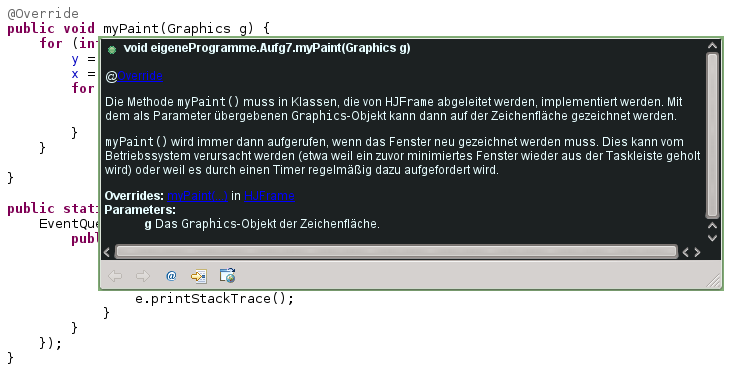
\includegraphics[width=1.0\textwidth]{./inf/SEKII/30_Java_Javadoc/HJFrame-Javadoc.png}
\end{center}
